% =============================================================================
% Integrantes: Arthur Meneses Neves, Danilo Oliveira Santos, Matheus Gabriel
% Viana Araujo, João Victor Vidal Barbosa, Guilherme Araujo Castro
%
% Síntese: Artigo final (Parte 3 / N2) do projeto da disciplina de
% Inteligência Artificial, no template SBC. Estende o artigo parcial
% (ArtigoParcial-Etapa2.tex) com: evolução da proposta, ajuste de
% hiperparâmetros com orçamento igual, conjunto ampliado de atributos e
% estudo de ablação, baseline por tabela idade x sexo, intervalos de
% confiança por bootstrap pareado, análise de erro por subgrupo com
% supressão de células pequenas, importância por permutação (XAI),
% checagem temporal e conclusão. Os números da N2 vêm do notebook 04 e dos
% arquivos em resultados/. Trechos marcados com \PEND{} aguardam a execução.
%
% Versões: sem RA (GitHub) por padrão; com RA e e-mail (AVA) se existir o
% arquivo docs/ras.tex, que não é versionado (ver .gitignore).
%
% Changelog:
%   2026-11-16 — Matheus Araujo — criação a partir do artigo parcial: nova
%     estrutura da N2 (contribuições alcançadas, resultados, conclusão),
%     metodologia da N2 e esqueleto dos resultados finais
% =============================================================================

\documentclass[12pt]{article}

\usepackage{sbc-template}
\usepackage{graphicx,url}
\usepackage[utf8]{inputenc}
\usepackage[brazilian]{babel}
\usepackage{xcolor}
\usepackage{tikz}
\usetikzlibrary{positioning,arrows.meta}

\sloppy

% Marca o que ainda depende da execução do notebook 04. Antes de entregar:
% grep -n PEND docs/ArtigoFinal-Etapa3.tex não deve devolver nada no corpo.
\newcommand{\PEND}[1]{\textcolor{red}{[#1]}}
% Figura gerada pelo notebook 04: enquanto não existir, mostra um aviso.
\newcommand{\figuraN}[2]{\IfFileExists{#2}{\includegraphics[#1]{#2}}{%
  \fbox{\parbox{0.8\textwidth}{\centering\PEND{figura \texttt{\detokenize{#2}}: rodar o notebook 04}}}}}

\title{Classificação da causa básica de óbito:\\
  uma comparação entre Random Forest e XGBoost}

\IfFileExists{ras.tex}{\input{ras.tex}}{%
\author{Arthur Meneses Neves, Danilo Oliveira Santos,\\
  Guilherme Araujo Castro, João Victor Vidal Barbosa,\\
  Matheus Gabriel Viana Araujo}}

\address{Faculdade de Computação e Informática (FCI)\\
Universidade Presbiteriana Mackenzie (UPM)\\
  São Paulo - SP - Brasil
  \ifdefined\emailsAVA\emailsAVA\fi
}

\begin{document}

\maketitle

\begin{resumo}
  Este artigo apresenta o resultado final de um projeto de IA aplicada que classifica a causa básica de óbito, agregada em seu capítulo da CID-10, a partir de atributos registrados na Declaração de Óbito e disponíveis no Sistema de Informação sobre Mortalidade (SIM), para o Brasil inteiro entre 2000 e 2026 (32.531.918 registros, 19 capítulos). Na primeira etapa, com cinco atributos sociodemográficos e configurações iniciais, Random Forest e XGBoost alcançaram F1-macro de 0,1329 e 0,1406, contra 0,0224 de um baseline de classe majoritária. Nesta etapa final, ajustamos os dois algoritmos com o mesmo orçamento de busca, comparamos o conjunto original de atributos com um conjunto ampliado (mês e ano do óbito, estado civil, local de ocorrência e assistência médica), introduzimos um baseline sem aprendizado (tabela idade $\times$ sexo) e medimos a incerteza por bootstrap pareado. O melhor modelo, \PEND{modelo}, alcança F1-macro de \PEND{0,xxxx} (IC 95\%: \PEND{0,xxxx}--\PEND{0,xxxx}). \PEND{Uma frase com a conclusão principal: o ganho veio dos atributos ou do ajuste? quanto acima da tabela idade×sexo?} Discutimos também o desempenho por subgrupo (sexo, raça/cor, faixa etária, escolaridade e região), a importância de cada atributo e as implicações éticas do uso desses modelos.
\end{resumo}

\section{Introdução}

\subsection{Contextualização}

O Sistema de Informação sobre Mortalidade (SIM) é o sistema do Ministério da Saúde que consolida as Declarações de Óbito emitidas no país. Seus microdados individuais estão disponíveis desde 1996, obtidos do DATASUS e publicados como dados abertos~\cite{pcdas_sim,sim_dadosgov}. Cada registro traz, além da causa básica do óbito codificada segundo a Classificação Internacional de Doenças, 10ª revisão (CID-10)~\cite{who_cid10}, atributos sociodemográficos do falecido e dados de residência e ocorrência.

A CID-10 organiza os códigos individuais em capítulos, que agrupam causas afins: doenças do aparelho circulatório, neoplasias, causas externas, e assim por diante. Trabalhar no nível de capítulo transforma a tarefa em um problema com poucas dezenas de classes, tratável com os algoritmos de aprendizado supervisionado vistos na disciplina. Este projeto trabalha com o recorte Brasil, âmbito nacional, período de 2000 a 2026.

\subsection{Justificativa}

Entender como fatores sociodemográficos e as circunstâncias do óbito se relacionam à categoria da causa é relevante para o planejamento de políticas públicas de saúde. O tema se alinha ao Objetivo de Desenvolvimento Sustentável 3 (Saúde e Bem-Estar), cuja meta 3.4 prevê reduzir em um terço, até 2030, a mortalidade prematura por doenças não transmissíveis~\cite{ods3}.

Há também uma justificativa metodológica. O SIM é uma base grande, pública e heterogênea entre anos, e a própria literatura registra limitações persistentes na qualidade do preenchimento das declarações de óbito~\cite{morais2017}. Medir quanto sinal existe nesses atributos, e reportar honestamente esse limite, é um resultado útil por si só, porque delimita o que se pode e o que não se pode esperar de modelos construídos sobre eles.

\subsection{Motivação}

A motivação do grupo combina três fatores: aplicar as técnicas de aprendizado de máquina da disciplina a um problema de saúde pública com impacto social claro; trabalhar com uma base pública de escala real, cujo volume obriga a lidar com questões práticas de engenharia de dados; e o fato de a tarefa ter desfecho incerto, já que não sabíamos, ao propor o projeto, quanto da causa de óbito seria previsível a partir desses atributos.

\subsection{Objetivo}

O objetivo é classificar a causa básica de óbito, agregada em seu capítulo da CID-10, a partir de atributos da Declaração de Óbito que não descrevem a causa, e medir quanto cada grupo de atributos contribui para essa classificação. Explicitamente:

\begin{itemize}
  \item Conjunto \emph{base} (o mesmo da N1): idade em anos completos, sexo, raça/cor, escolaridade e unidade da federação de residência.
  \item Conjunto \emph{ampliado} (N2): o conjunto base mais mês e ano do óbito, estado civil, local de ocorrência e se houve assistência médica durante a doença que levou ao óbito.
  \item Variável de saída: o capítulo da CID-10 da causa básica, com $k = 19$ classes observadas (capítulos I a XVIII e XX; os capítulos XIX e XXI nunca ocorrem como causa básica nesta base), listadas na Tabela~\ref{tab:classes}.
  \item Período e região: 2000 a 2026 (2026 parcial), Brasil, âmbito nacional.
\end{itemize}

Nenhuma variável que descreva a cadeia de causas da própria declaração é usada como entrada, para evitar vazamento do rótulo. A Seção~\ref{sec:metodologia} detalha como isso é garantido e verificado em código.

\subsection{Contribuições alcançadas}

\begin{itemize}
  \item Uma análise exploratória e uma preparação documentadas e reprodutíveis do SIM 2000--2026, incluindo as inconsistências de formato entre anos (arquivos sem cabeçalho, três formatos de data) e a evolução do não-preenchimento, com testes automatizados para cada regra de preparação.
  \item Uma comparação entre Random Forest e XGBoost sob o mesmo protocolo e o mesmo orçamento de ajuste, com intervalos de confiança e testes de diferença pareados, e contra dois baselines, um deles sem aprendizado de máquina (tabela idade $\times$ sexo).
  \item Uma medida da contribuição de cada grupo de atributos (sociodemográfico, tempo, estado civil, circunstância do óbito) por ablação e por importância por permutação, que testa a hipótese da N1 de que o limite vinha dos atributos e não do algoritmo. \PEND{confirmar se a hipótese se sustentou}
  \item Uma análise de desempenho por subgrupo (sexo, raça/cor, faixa etária, escolaridade e região), com supressão de células pequenas implementada em código.
\end{itemize}

\section{Fundamentação Teórica e Trabalhos Relacionados}

\subsection{Conceitos fundamentais}

O problema é de classificação supervisionada multiclasse: dado um vetor de atributos $x$, atribuir a ele um rótulo $y$ entre $k$ classes mutuamente exclusivas, aprendendo a associação a partir de exemplos rotulados. Os dois algoritmos comparados pertencem à família dos \emph{ensembles} de árvores de decisão.

Random Forest~\cite{breiman2001} treina um conjunto de árvores de decisão, cada uma sobre uma amostra bootstrap dos dados e com uma seleção aleatória de atributos em cada nó; a predição final é o voto da maioria. A aleatorização reduz a correlação entre as árvores, e o erro de generalização da floresta depende da força das árvores individuais e dessa correlação. É robusto a atributos irrelevantes e de treino paralelizável.

XGBoost~\cite{chen2016} implementa \emph{gradient boosting}: as árvores são construídas em sequência, cada uma ajustada ao erro residual das anteriores, com regularização explícita da complexidade. O trabalho original descreve um algoritmo consciente de esparsidade e um esquema aproximado de busca de pontos de corte baseado em quantis ponderados (\emph{weighted quantile sketch}), além de otimizações de acesso a cache, compressão e particionamento. Na implementação usada aqui, o método \texttt{hist} agrupa os valores de cada atributo em histogramas, o que torna o treino viável com dezenas de milhões de linhas.

Desbalanceamento de classes: quando uma classe domina a base, a acurácia deixa de ser informativa, porque um classificador trivial que sempre prevê a classe majoritária já a maximiza. Por isso adotamos o F1-macro, a média simples do F1 de cada classe, que dá o mesmo peso a um capítulo com 8,8 milhões de registros e a um com 629, além do recall por classe e da matriz de confusão.

Vazamento de rótulo (\emph{label leakage}) é a presença, entre os atributos, de informação que só existe porque o rótulo já é conhecido. Em declarações de óbito o risco é concreto: os campos da cadeia de causas são o próprio rótulo em outra forma. Há também o vazamento indireto, quando um atributo é consequência da causa; é o caso da indicação de necropsia, discutido na Seção~\ref{sec:metodologia}.

Ajuste de hiperparâmetros: a busca aleatória~\cite{bergstra2012} sorteia configurações de um espaço definido e, com o mesmo número de tentativas, tende a encontrar configurações tão boas quanto a busca em grade, porque poucos hiperparâmetros costumam importar. Para comparar dois algoritmos de forma justa, os dois recebem o mesmo número de tentativas e são avaliados em um conjunto de validação separado do teste.

Incerteza: o bootstrap~\cite{efron1993} reamostra o conjunto de teste com reposição para estimar a variabilidade de uma métrica. No bootstrap \emph{pareado}, todos os modelos são avaliados nas mesmas reamostragens, o que permite obter um intervalo de confiança para a \emph{diferença} entre eles.

Para explicabilidade, usamos a importância por permutação~\cite{breiman2001,fisher2019}, que mede quanto o desempenho cai quando os valores de um atributo são embaralhados, desfazendo sua relação com o rótulo sem alterar sua distribuição. É independente do modelo e, aplicada às colunas originais (antes do \emph{one-hot}), mede a importância do atributo inteiro.

Viés e equidade: um modelo pode ter desempenho desigual entre grupos da população, seja porque os dados representam esses grupos de forma desigual, seja porque a qualidade do registro difere entre eles~\cite{mehrabi2021}. Medir o desempenho por subgrupo é o primeiro passo para identificar esse problema.

A implementação usa scikit-learn~\cite{pedregosa2011} (versão 1.9.1) e XGBoost (versão 3.4.1).

\subsection{Trabalhos relacionados}

\cite{mujtaba2017} classificaram automaticamente a causa de óbito em 9 categorias da CID-10 a partir do texto livre de 2.200 laudos de necropsia relacionados a acidentes. Compararam cinco classificadores (Naive Bayes, SVM, k-NN, J48 e Random Forest) com seis estratégias de seleção de atributos; a melhor solução foi o Random Forest com seleção guiada por especialistas, com cerca de 90\% de acurácia e de F-medida macro. O alto desempenho vem de entradas que \emph{descrevem clinicamente o óbito} (exame externo, lesões, histórico médico). Lá, o problema é automatizar a codificação a partir da descrição clínica; aqui, medir a associação entre o perfil do falecido e a categoria de causa, sem nenhuma informação clínica.

\cite{silva2022} compararam Regressão Logística, Árvore de Decisão e Random Forest para prever óbito por COVID-19 a partir de dados clínicos de 134.639 pacientes do SUS em 2021; o melhor foi o Random Forest, com 77\% de acurácia e AUC-ROC de 0,75, tendo suporte ventilatório, UTI, idade e comorbidades como fatores mais importantes. \cite{santos2019} aplicaram cinco algoritmos a 2.808 idosos do estudo SABE, em São Paulo, para predizer óbito em cinco anos a partir de 37 preditores demográficos, socioeconômicos e de saúde; todos superaram AUC-ROC de 0,70.

\cite{morais2017} avaliaram o próprio SIM como sistema de informação, com 45 indicadores de qualidade aplicados a profissionais e gestores de saúde no nordeste de São Paulo. Cerca de 47\% dos usuários relataram algum grau de informação incorreta, especialmente na causa de óbito. Esse achado sustenta a decisão de tratar ``ignorado'' como categoria explícita em vez de imputá-lo.

A Tabela~\ref{tab:relacionados} resume as diferenças. Os trabalhos de melhor desempenho usam informação clínica, e os de desfecho binário têm tarefa intrinsecamente mais fácil que a nossa (19 classes). Deles retiramos três decisões: comparar mais de um algoritmo sob o mesmo protocolo, relatar métricas que não dependam só da acurácia e, de \cite{silva2022}, examinar quais atributos o modelo usa. A limitação comum a todos, e que este trabalho procura evitar, é reportar um único número de desempenho sem intervalo de confiança nem análise por subgrupo. Nenhum dos trabalhos classifica a categoria da causa entre óbitos já registrados, em escala nacional e em série histórica longa, usando apenas atributos não clínicos do SIM.

\begin{table}[ht]
\centering
\caption{Comparação com os trabalhos relacionados.}
\label{tab:relacionados}
\resizebox{\textwidth}{!}{%
\begin{tabular}{|l|l|l|l|l|}
\hline
\textbf{Trabalho} & \textbf{Tarefa} & \textbf{Entradas} & \textbf{Dados} & \textbf{Melhor resultado} \\
\hline
\cite{mujtaba2017} & 9 categorias CID-10 & texto de necropsia & 2.200 laudos & RF, F1-macro $\approx$ 0,90 \\
\cite{silva2022} & óbito COVID (binário) & clínicas & 134.639 & RF, AUC 0,75 \\
\cite{santos2019} & óbito em 5 anos (binário) & 37 mistas & 2.808 & AUC $>$ 0,70 \\
Este trabalho & 19 capítulos CID-10 & 5 a 10 não clínicas & 32,5 milhões & \PEND{modelo, F1-macro} \\
\hline
\end{tabular}}
\end{table}

\section{Metodologia e Resultados Esperados}
\label{sec:metodologia}

\subsection{Evolução em relação à proposta e à primeira etapa}

A proposta inicial previa comparar Random Forest e XGBoost sobre atributos sociodemográficos. A primeira etapa (N1) cumpriu isso com configurações iniciais e terminou com seis limitações explícitas: (i) uma divisão e uma semente, sem intervalo de confiança; (ii) hiperparâmetros não ajustados e profundidades diferentes entre os modelos; (iii) conclusões sobre os capítulos VII e VIII apoiadas em poucos casos; (iv) ausência de análise por subgrupo; (v) a decisão de mapear o código 0 de escolaridade para ``ignorado''; e (vi) a supressão de células pequenas ainda não implementada. A N1 também levantou uma hipótese: ``o limite observado parece vir do conjunto de atributos, não da escolha do algoritmo''.

A etapa final foi desenhada para responder a cada ponto. Para (ii) e para a hipótese, separamos dois efeitos: o do \emph{ajuste} (mesmo conjunto base, hiperparâmetros ajustados) e o dos \emph{atributos} (conjunto ampliado, mesmos hiperparâmetros). As demais limitações são tratadas por bootstrap pareado e repetição com sementes (i), amostras com piso por classe e suporte reportado ao lado de cada resultado (iii), análise por subgrupo (iv), contagem de \texttt{ESC = 0} por ano (v) e uma função de supressão aplicada a todas as tabelas por subgrupo (vi). O escopo não mudou: mesmo alvo, mesmo período, mesma região e o mesmo conjunto de teste da N1.

\subsection{Arquitetura e etapas}

A Figura~\ref{fig:arquitetura} mostra o fluxo. O código está organizado em quatro notebooks (\texttt{01\_eda\_exploratoria}, \texttt{02\_preparacao\_dados}, \texttt{03\_resultados\_parciais} e \texttt{04\_resultados\_finais}) e dois módulos (\texttt{src/sim\_utils.py}, leitura e preparação; \texttt{src/avaliacao.py}, avaliação), cobertos por 54 testes automatizados.

\begin{figure}[ht]
\centering
\begin{tikzpicture}[
  caixa/.style={draw, rounded corners, align=center, font=\scriptsize, minimum height=0.9cm, text width=2.35cm},
  seta/.style={-{Stealth}, thick}, node distance=0.35cm]
\node[caixa] (csv) {27 CSVs do SIM\\2000--2026};
\node[caixa, right=of csv] (prep) {Leitura e preparação\\(\texttt{sim\_utils})\\cache Parquet};
\node[caixa, right=of prep] (split) {Divisão 80/20\\estratificada\\(igual à N1)};
\node[caixa, right=of split] (busca) {Busca aleatória\\RF e XGBoost\\(validação)};
\node[caixa, below=0.7cm of busca] (final) {Modelos finais\\base e ampliado};
\node[caixa, left=of final] (aval) {Teste: F1-macro,\\IC bootstrap,\\por classe};
\node[caixa, left=of aval] (sub) {Subgrupos\\(supressão $<$10)\\e permutação};
\node[caixa, left=of sub] (temp) {Checagem\\temporal\\($\le$2022 $\to$ 2023+)};
\draw[seta] (csv) -- (prep);
\draw[seta] (prep) -- (split);
\draw[seta] (split) -- (busca);
\draw[seta] (busca) -- (final);
\draw[seta] (final) -- (aval);
\draw[seta] (aval) -- (sub);
\draw[seta] (sub) -- (temp);
\end{tikzpicture}
\caption{Fluxo da solução. O conjunto de teste só é usado a partir dos modelos finais.}
\label{fig:arquitetura}
\end{figure}

\begin{enumerate}
  \item Análise exploratória (notebook 01) e preparação (notebook 02, ampliada na N2 com as novas colunas).
  \item Divisão treino/teste: a mesma da N1, aleatória e estratificada por classe, 80\% para treino e 20\% (6.506.384 linhas) para teste.
  \item Busca de hiperparâmetros: \PEND{10} configurações sorteadas para cada algoritmo, treinadas em uma amostra estratificada de \PEND{1.000.000} linhas do treino e avaliadas por F1-macro em uma validação de \PEND{500.000} linhas, também tirada do treino e disjunta da amostra de busca. As amostras têm piso de 50 linhas por classe, para que os capítulos VII e VIII estejam presentes. Os espaços de busca estão no notebook 04; no Random Forest a profundidade foi limitada a 16, porque com 19 classes cada nó armazena 19 valores e árvores sem limite não caberiam em memória no treino final.
  \item Variação por semente: os melhores modelos são retreinados com 3 sementes, mudando também a amostra de treino.
  \item Ablação: o XGBoost ajustado é treinado com os grupos de atributos entrando de forma cumulativa e com cada grupo retirado do conjunto ampliado.
  \item Modelos finais: Random Forest e XGBoost com os melhores parâmetros, nos conjuntos base e ampliado, treinados com \PEND{30\%} do treino (amostra estratificada de \PEND{7,8} milhões de linhas) e avaliados no teste completo.
  \item Avaliação no teste: F1-macro com intervalo de confiança de 95\% por bootstrap pareado (\PEND{200} réplicas), métricas por classe, matriz de confusão, desempenho por subgrupo, importância por permutação e checagem temporal (treino até 2022, teste 2023 a 2026).
\end{enumerate}

Dois baselines servem de referência: o de classe majoritária, da N1, e uma \emph{tabela idade $\times$ sexo}, que, para cada faixa de 5 anos e sexo, prevê a classe de maior frequência ponderada pelos mesmos pesos balanceados dos modelos. A tabela não usa aprendizado de máquina; se um modelo não a supera, ele não aprendeu nada além de uma regra de idade e sexo.

O desbalanceamento é tratado com pesos de amostra balanceados, iguais para os dois algoritmos, como na N1. Essa escolha sacrifica acurácia nas classes frequentes em troca de recall nas raras, e por isso a acurácia entra apenas como referência.

A prevenção de vazamento de rótulo é estrutural e verificada. Estrutural, porque a leitura dos CSVs carrega apenas as colunas listadas na Tabela~\ref{tab:colunas}, e os campos da cadeia de causas nunca entram em memória. Verificada, porque testes automatizados falham se alguma entrada for o rótulo, um campo da cadeia de causas ou a necropsia. A necropsia ficou de fora por vazamento indireto: ela é indicada quando se suspeita de morte violenta, portanto é consequência da causa. O local de ocorrência exige mais cuidado: ``via pública'' está associado a causas externas, mas é uma informação observada no momento do óbito, registrada no bloco de ocorrência da declaração e não derivada da causa codificada. Por isso ele entra no modelo, e a ablação mede separadamente quanto do ganho depende dele.

\subsection{Dataset}
\label{sec:dataset}

Os arquivos ``Mortalidade Geral'' do SIM foram obtidos no Portal Brasileiro de Dados Abertos (\url{https://dados.gov.br/dados/conjuntos-dados/sim-1979-2019})~\cite{sim_dadosgov} e cobrem 2000--2026, conforme registrado em \texttt{data/README.md}. São arquivos CSV separados por ponto e vírgula, em \texttt{latin1}, um por ano. Cada registro é uma Declaração de Óbito. O número de colunas cresce de 39 (2000) para 88 (2024) ao longo da série. Este projeto lê as colunas da Tabela~\ref{tab:colunas}; as três colunas novas da N2 são lidas nos anos em que existem e viram ``Ignorado'' nos demais.

\begin{table}[ht]
\centering
\caption{Colunas lidas dos arquivos brutos e seu papel no projeto.}
\label{tab:colunas}
\small
\begin{tabular}{|l|l|l|}
\hline
\textbf{Coluna} & \textbf{Significado} & \textbf{Papel} \\
\hline
\texttt{IDADE} & Idade codificada (unidade + valor) & Entrada (anos) \\
\texttt{SEXO} & 0 ignorado, 1 masculino, 2 feminino & Entrada \\
\texttt{RACACOR} & Raça/cor autodeclarada (1 a 5) & Entrada \\
\texttt{ESC} & Escolaridade (1 a 5, 9 ignorado) & Entrada \\
\texttt{CODMUNRES} & Município de residência (IBGE) & Entrada (agregada em UF) \\
\texttt{DTOBITO} & Data do óbito & Entrada ampliada (mês) \\
\texttt{ESTCIV} & Estado civil & Entrada ampliada (N2) \\
\texttt{LOCOCOR} & Local de ocorrência & Entrada ampliada (N2) \\
\texttt{ASSISTMED} & Assistência médica na doença & Entrada ampliada (N2) \\
\texttt{CAUSABAS} & Causa básica (CID-10) & Rótulo (capítulo) \\
\texttt{TIPOBITO} & 1 fetal, 2 não fetal & Só verificação \\
\hline
\end{tabular}
\end{table}

A análise exploratória (notebook 01) revelou problemas de qualidade que definiram a preparação: formatos divergentes entre anos (os arquivos de 2022 e 2023 não têm cabeçalho, e a data aparece em três formatos), dois tipos de ``sem informação'' (o valor ausente e o código 9), não-preenchimento que muda muito ao longo do tempo (Figura~\ref{fig:ausentes}) e mudança na composição das causas.

\begin{figure}[ht]
\centering
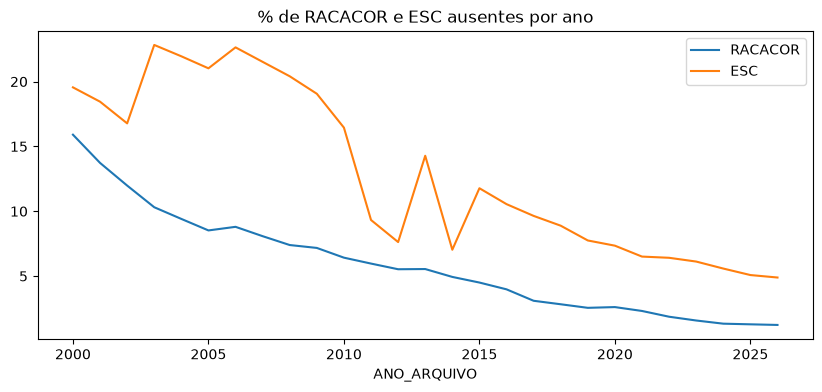
\includegraphics[width=0.95\textwidth]{figuras/ausentes_por_ano.png}
\caption{Percentual de registros com \texttt{RACACOR} e \texttt{ESC} ausentes, por ano (2000-2026). O código 9 (``ignorado''), que é um valor preenchido, não aparece nesta contagem e é tratado à parte.}
\label{fig:ausentes}
\end{figure}

A preparação é feita por uma única função, compartilhada por todos os notebooks, e seu resultado fica em um cache Parquet cuja chave inclui o tamanho e a data de modificação de cada CSV e uma constante de versão, de modo que um cache desatualizado nunca é usado. As decisões foram:

\begin{itemize}
  \item Idade: decodificada para anos completos a partir do código do SIM (o primeiro dígito indica a unidade e os dois últimos, o valor).
  \item Escolaridade, raça/cor, estado civil, local de ocorrência e assistência médica: mapeadas para categorias nomeadas, com ``Ignorado'' como categoria explícita em vez de imputação. ``Ignorado'' soma 26,409\% em \texttt{ESC} e 5,389\% em \texttt{RACACOR}; descartar essas linhas enviesaria a amostra contra os anos iniciais. \PEND{percentuais de Ignorado de ESTCIV, LOCOCOR e ASSISTMED (n2\_ignorado\_por\_ano.csv)}
  \item Código 0 de escolaridade: não consta do dicionário de \texttt{ESC} e foi mapeado para ``Ignorado''. Na N2, contamos sua ocorrência por ano: \PEND{x\% do bruto, concentrado em ... (n2\_esc\_zero\_por\_ano.csv)}, o que \PEND{sustenta / não sustenta} a decisão.
  \item Mês do óbito: extraído de \texttt{DTOBITO} depois de normalizar os três formatos de data; data inválida vira ``Ignorado''.
  \item Município: truncado para 6 dígitos e agregado em unidade da federação. Com mais de 5.500 municípios, o \emph{one-hot} seria inviável e o risco de reidentificação em células pequenas aumentaria (Seção~\ref{sec:etica}).
  \item Filtros: foram descartados 15.842 registros com \texttt{SEXO} ignorado, 81.308 com idade desconhecida e 3 sem capítulo da CID-10 (97.153 no total, 0,2977\% do bruto), restando 32.531.918 registros e 19 classes.
\end{itemize}

A Tabela~\ref{tab:classes} e a Figura~\ref{fig:distribuicao} mostram as 19 classes. O capítulo IX (circulatório) concentra 27,0141\% dos registros, e o capítulo VII (olho), 0,0019\%, uma razão de 13.972 entre o maior e o menor. Com 19 classes e esse desbalanceamento, são necessários baselines explícitos, pesos balanceados e métricas macro-agregadas para que o resultado signifique alguma coisa.

\begin{table}[ht]
\centering
\caption{Distribuição do alvo: capítulos da CID-10 observados em 32.531.918 registros (SIM, Brasil, 2000-2026).}
\label{tab:classes}
\small
\begin{tabular}{|l|l|r|r|}
\hline
\textbf{Cap.} & \textbf{Descrição} & \textbf{Registros} & \textbf{\%} \\
\hline
IX    & Doenças do aparelho circulatório                       & 8.788.199 & 27,0141 \\
II    & Neoplasias (tumores)                                   & 5.108.490 & 15,7030 \\
XX    & Causas externas de morbidade e mortalidade             & 3.712.335 & 11,4114 \\
X     & Doenças do aparelho respiratório                       & 3.516.512 & 10,8094 \\
XVIII & Sintomas, sinais e causas mal definidas                & 2.328.478 &  7,1575 \\
I     & Doenças infecciosas e parasitárias                     & 2.108.449 &  6,4812 \\
IV    & Doenças endócrinas, nutricionais e metabólicas         & 1.896.126 &  5,8285 \\
XI    & Doenças do aparelho digestivo                          & 1.614.124 &  4,9617 \\
XIV   & Doenças do aparelho geniturinário                      &   879.273 &  2,7028 \\
VI    & Doenças do sistema nervoso                             &   854.902 &  2,6279 \\
XVI   & Afecções originadas no período perinatal               &   632.965 &  1,9457 \\
V     & Transtornos mentais e comportamentais                  &   336.307 &  1,0338 \\
XVII  & Malformações congênitas e anomalias cromossômicas      &   271.194 &  0,8336 \\
III   & Doenças do sangue e transtornos imunitários            &   165.129 &  0,5076 \\
XII   & Doenças da pele e do tecido subcutâneo                 &   134.961 &  0,4149 \\
XIII  & Doenças do sistema osteomuscular e tecido conjuntivo   &   132.556 &  0,4075 \\
XV    & Gravidez, parto e puerpério                            &    46.798 &  0,1439 \\
VIII  & Doenças do ouvido e da apófise mastoide                &     4.491 &  0,0138 \\
VII   & Doenças do olho e anexos                               &       629 &  0,0019 \\
\hline
\end{tabular}
\end{table}

\begin{figure}[ht]
\centering
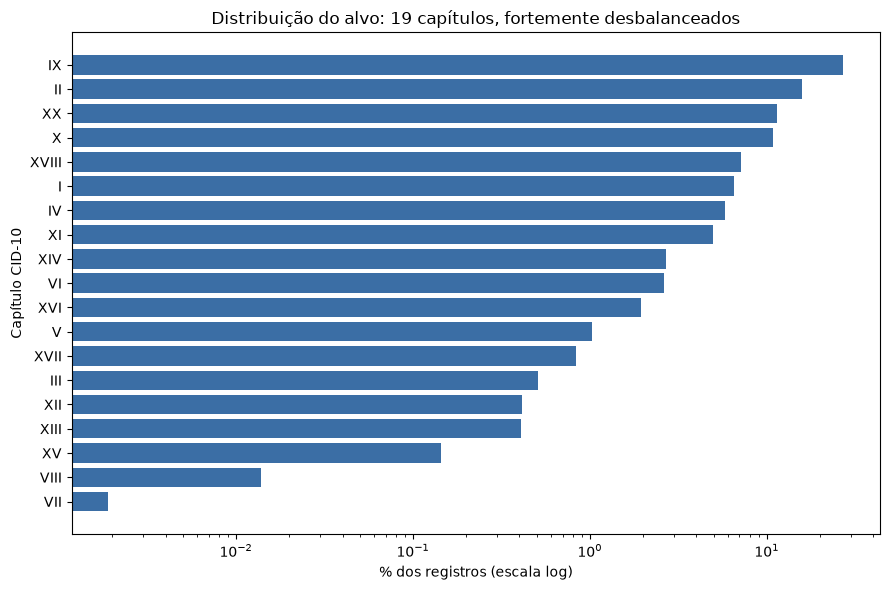
\includegraphics[width=0.85\textwidth]{figuras/distribuicao_capitulos.png}
\caption{Participação de cada capítulo da CID-10 no total de registros, em escala logarítmica. Os capítulos XIX e XXI não aparecem porque nunca ocorrem como causa básica nesta base.}
\label{fig:distribuicao}
\end{figure}

\subsection{Resultados esperados}

Com base na N1, esperávamos que o ajuste de hiperparâmetros trouxesse ganho pequeno e que os atributos novos trouxessem ganho maior, concentrado nos capítulos ligados à circunstância (causas externas, pelo local de ocorrência) e à sazonalidade (respiratório, pelo mês). Também esperávamos que os modelos superassem a tabela idade $\times$ sexo, mas com margem menor do que a margem sobre o baseline de classe majoritária. A Seção~\ref{sec:resultados} mostra \PEND{o que de fato ocorreu}.

\section{Resultados}
\label{sec:resultados}

\subsection{Aspectos éticos e responsabilidade no uso da IA}
\label{sec:etica}

\textbf{Privacidade.} O projeto usa exclusivamente os microdados públicos do SIM, publicados como dados abertos sob licença CC-BY. Nenhuma coluna lida é identificador direto. A LGPD~\cite{lgpd} define dado anonimizado como aquele ``relativo a titular que não possa ser identificado, considerando a utilização de meios técnicos razoáveis e disponíveis na ocasião de seu tratamento'' (art.~5º, III) e estabelece, no art.~12, que ele não é dado pessoal, \emph{salvo} quando a anonimização puder ser revertida com esforços razoáveis. A combinação de quase-identificadores (idade, município, data do óbito, estado civil) pode permitir reidentificação em municípios pequenos ou para causas raras. Medidas adotadas: o município entra apenas como UF; nenhuma tabela publicada desce ao nível de município ou de data; e todas as tabelas por subgrupo passam por uma função que suprime métricas e contagens de células com menos de 10 casos (\texttt{avaliacao.suprimir\_celulas\_pequenas}), limitação que a N1 deixou em aberto.

\textbf{Vazamento e honestidade dos resultados.} Um modelo que acertasse a causa porque leu a descrição da causa não mediria associação nenhuma. A exclusão estrutural da cadeia de causas e da necropsia, verificada por testes, e a ablação que separa o efeito do local de ocorrência são, portanto, também uma exigência de honestidade na apresentação dos resultados.

\textbf{Viés.} O não-preenchimento de raça/cor e escolaridade é grande e varia ao longo dos anos (Figura~\ref{fig:ausentes}); mantemos ``Ignorado'' como categoria explícita em vez de imputar, o que esconderia o viés em vez de expô-lo. A análise por subgrupo (Seção~\ref{sec:desempenho}) mostra \PEND{resumo: amplitude do F1-macro entre grupos de raça/cor, escolaridade e região; algum grupo claramente pior?}. Diferenças entre subgrupos não são, sozinhas, prova de viés do modelo, porque a composição de causas difere entre grupos; por isso comparamos cada subgrupo também com a tabela idade $\times$ sexo. \PEND{interpretação}

\textbf{Uso pretendido e limites.} O objetivo é apoiar o planejamento em saúde pública em nível agregado, por exemplo, estimar a composição esperada de causas para um perfil populacional. O modelo não deve ser usado para decisões sobre pessoas, nem para inferir a causa de uma morte específica sem o laudo médico, que é a fonte de verdade. O desempenho absoluto (F1-macro de \PEND{0,xx}) reforça essa restrição. O alvo é o capítulo da CID-10, e não o código completo, o que produz uma categoria ampla e auditável. Todo o código, incluindo a preparação e as verificações de vazamento, é público.

\textbf{Comitê de ética.} O projeto usa apenas dados públicos, secundários e anonimizados, sem acesso a registros identificáveis, sem vinculação com outras bases e sem contato com pessoas; nessas condições, em linha com a orientação da disciplina, o grupo conclui que a submissão ao CEP não é necessária. Isso deve ser reavaliado se o projeto passar a usar registros identificáveis, cruzar o SIM com outra base ou envolver contato com pessoas.

\subsection{Detalhamento dos resultados}
\label{sec:desempenho}

\textbf{Ajuste de hiperparâmetros.} A Tabela~\ref{tab:hiper} mostra as melhores configurações. \PEND{comentar: o ajuste mudou muito em relação às configurações da N1 (RF profundidade 12; XGB 100 rodadas, profundidade 6, taxa 0,3)? Quanto ganhou na validação?} A variação entre as 3 sementes foi de \PEND{desvio-padrão} no Random Forest e \PEND{desvio-padrão} no XGBoost, \PEND{menor/maior} que a diferença entre os dois algoritmos.

\begin{table}[ht]
\centering
\caption{Melhores hiperparâmetros encontrados pela busca aleatória (\PEND{10} configurações por algoritmo) e F1-macro na validação.}
\label{tab:hiper}
\small
\begin{tabular}{|l|l|r|}
\hline
\textbf{Modelo} & \textbf{Hiperparâmetros} & \textbf{F1-macro val.} \\
\hline
Random Forest & \PEND{n\_estimators, max\_depth, min\_samples\_leaf, max\_features} & \PEND{} \\
XGBoost & \PEND{n\_estimators, max\_depth, learning\_rate, ...} & \PEND{} \\
\hline
\end{tabular}
\end{table}

\textbf{Comparação no teste.} A Tabela~\ref{tab:comparacao} reúne os baselines, os modelos da N1 e os quatro modelos finais.

\begin{table}[ht]
\centering
\caption{Desempenho no conjunto de teste (6.506.384 linhas, a mesma divisão da N1). IC 95\% por bootstrap pareado. A acurácia consta apenas como referência.}
\label{tab:comparacao}
\small
\begin{tabular}{|l|r|r|r|r|}
\hline
\textbf{Modelo} & \textbf{F1-macro} & \textbf{IC 95\%} & \textbf{Acurácia} & \textbf{Treino (s)} \\
\hline
Baseline classe majoritária & 0,0224 & -- & 0,2701 & -- \\
Baseline tabela idade $\times$ sexo & \PEND{} & \PEND{} & \PEND{} & \PEND{} \\
Random Forest N1 (sem ajuste) & 0,1329 & -- & 0,1625 & 343,9 \\
XGBoost N1 (sem ajuste) & 0,1406 & -- & 0,1755 & 983,3 \\
\hline
Random Forest ajustado, base & \PEND{} & \PEND{} & \PEND{} & \PEND{} \\
XGBoost ajustado, base & \PEND{} & \PEND{} & \PEND{} & \PEND{} \\
Random Forest ajustado, ampliado & \PEND{} & \PEND{} & \PEND{} & \PEND{} \\
XGBoost ajustado, ampliado & \PEND{} & \PEND{} & \PEND{} & \PEND{} \\
\hline
\end{tabular}
\end{table}

\PEND{Discussão em 3 parágrafos, com os números de n2\_diferencas.csv: (1) efeito do ajuste: modelos base ajustados vs. N1; (2) efeito dos atributos: ampliado vs. base, com IC da diferença; (3) RF vs. XGBoost: a diferença é maior que o ruído entre sementes? o custo compensa? (4) margem sobre a tabela idade×sexo. Nota: os modelos da N1 foram treinados com 100\% do treino e os da N2 com a fração indicada; dizer isso ao comparar.}

\textbf{Ablação e importância dos atributos.} A Tabela~\ref{tab:ablacao} mostra o ganho de cada grupo, e a Figura~\ref{fig:importancia}, a importância por permutação no melhor modelo. \PEND{Qual grupo trouxe mais ganho? Quanto do ganho depende do local de ocorrência? A hipótese da N1 se confirmou?}

\begin{table}[ht]
\centering
\caption{Ablação dos grupos de atributos (XGBoost ajustado, F1-macro na validação).}
\label{tab:ablacao}
\small
\begin{tabular}{|l|r|r|}
\hline
\textbf{Conjunto} & \textbf{F1-macro val.} & \textbf{Variação} \\
\hline
Base (sociodemográfico) & \PEND{} & -- \\
+ tempo (mês, ano) & \PEND{} & \PEND{} \\
+ estado civil & \PEND{} & \PEND{} \\
+ circunstância (local, assistência) & \PEND{} & \PEND{} \\
\hline
Ampliado sem tempo & \PEND{} & \PEND{} \\
Ampliado sem estado civil & \PEND{} & \PEND{} \\
Ampliado sem circunstância & \PEND{} & \PEND{} \\
\hline
\end{tabular}
\end{table}

\begin{figure}[ht]
\centering
\figuraN{width=0.7\textwidth}{figuras/n2_importancia.png}
\caption{Importância por permutação: queda do F1-macro ao embaralhar cada atributo, em uma amostra de \PEND{300.000} linhas do teste.}
\label{fig:importancia}
\end{figure}

\textbf{Desempenho por classe.} A Figura~\ref{fig:f1classe} compara o F1 por capítulo da tabela idade $\times$ sexo e do XGBoost nos dois conjuntos. \PEND{Quais capítulos melhoraram com os atributos novos (esperado: XX pelo local, X pelo mês)? Quais continuam perto de zero? Capítulos VII e VIII: lembrar o suporte (126 e 898).}

\begin{figure}[ht]
\centering
\figuraN{width=\textwidth}{figuras/n2_f1_por_classe.png}
\caption{F1 por capítulo no teste, ordenado pelo número de casos.}
\label{fig:f1classe}
\end{figure}

\textbf{Subgrupos.} A Figura~\ref{fig:subgrupos} mostra o F1-macro do melhor modelo por subgrupo, com a tabela idade $\times$ sexo como referência. \PEND{descrever as maiores diferenças e se o ganho sobre a tabela é parecido entre grupos.}

\begin{figure}[ht]
\centering
\figuraN{width=\textwidth}{figuras/n2_subgrupos.png}
\caption{F1-macro do melhor modelo por subgrupo (barras) e da tabela idade $\times$ sexo (traços). Células com menos de 10 casos são suprimidas.}
\label{fig:subgrupos}
\end{figure}

\textbf{Generalização temporal.} Treinando até 2022 e testando em 2023, 2024, 2025 e 2026, \PEND{resultado; comparar com a N1, em que o F1-macro caiu 0,0051 (RF) e 0,0053 (XGBoost) entre 2023 e 2026}.

\textbf{Limitações.} \PEND{revisar ao final} (i) os modelos finais foram treinados com uma fração do treino por limite de memória; (ii) o intervalo de confiança do bootstrap mede a incerteza do teste, e a do treino é estimada só por 3 sementes; (iii) os capítulos VII e VIII continuam com poucos casos de teste; (iv) a busca de hiperparâmetros cobre \PEND{10} configurações por algoritmo, longe de um ajuste exaustivo; (v) o local de ocorrência, embora não derivado da causa, está fortemente associado a causas externas, e um uso do modelo que não tenha essa informação disponível deve usar o conjunto base.

\subsection{Endereços do repositório e do vídeo}

Todo o material está em um repositório público: \url{https://github.com/araujoviana/projeto1-IA-2026}. Ele contém este artigo (fontes LaTeX e PDF), a descrição do dataset e o procedimento para obtê-lo (\texttt{data/README.md}), os quatro notebooks executados, os módulos de funções com testes automatizados, os resultados exportados em \texttt{resultados/} e o histórico de alterações no Git. O vídeo de apresentação está em \PEND{\url{https://youtu.be/...}}.

\section{Conclusão}

Este projeto classificou o capítulo da CID-10 da causa básica de óbito a partir de atributos não clínicos da Declaração de Óbito, usando 32,5 milhões de registros do SIM (2000--2026). Na primeira etapa, com cinco atributos sociodemográficos, Random Forest e XGBoost superaram com folga o baseline de classe majoritária, mas com F1-macro baixo em termos absolutos (0,13 a 0,14). Na etapa final, ajustamos os dois algoritmos com o mesmo orçamento, ampliamos o conjunto de atributos e medimos a incerteza e o desempenho por subgrupo.

\PEND{Parágrafo com o resultado principal: melhor modelo e F1-macro com IC; quanto veio do ajuste e quanto dos atributos; margem sobre a tabela idade×sexo; RF vs. XGBoost.}

\PEND{Parágrafo sobre o objetivo: foi alcançado? Classificar com o desempenho medido e, principalmente, medir quanto cada grupo de atributos contribui. Responder à hipótese da N1.}

As contribuições efetivas são: uma preparação reprodutível e testada do SIM em série longa; uma comparação entre algoritmos com intervalos de confiança e baselines que tornam o resultado interpretável; a medida da contribuição de cada grupo de atributos; e uma análise de desempenho por subgrupo com proteção de células pequenas. O resultado também tem valor negativo: atributos não clínicos explicam pouco da causa do óbito, e qualquer uso desses modelos deve ser agregado, nunca individual. Como trabalhos futuros, sugerimos incorporar variáveis agregadas por município (porte, cobertura de atenção básica), com supressão de células pequenas, e avaliar limiares de decisão por classe, que podem melhorar o equilíbrio entre precisão e recall nos capítulos raros.

\bibliographystyle{sbc}
\bibliography{referencias}

\end{document}
